\documentclass[11pt,a4paper]{article}

\usepackage[margin=1in]{geometry}
\usepackage{mathptmx}
\usepackage{amsmath}
\usepackage{amssymb}
\usepackage{amsthm}
\usepackage{braket}
\usepackage{tikz}
\usepackage{quantikz}
\usepackage{enumitem}
\usepackage{hyperref}
\usepackage{xcolor}

\definecolor{circuitblue}{RGB}{40,80,160}

\hypersetup{
    colorlinks=true,
    linkcolor=circuitblue,
    urlcolor=circuitblue,
    citecolor=circuitblue
}

\theoremstyle{definition}
\newtheorem{definition}{Definition}[section]
\newtheorem{example}{Example}[section]

\theoremstyle{remark}
\newtheorem*{intuition}{Intuition}
\newtheorem*{keypoint}{Key Point}

\pagestyle{plain}

\setlength{\parindent}{0pt}
\setlength{\parskip}{6pt}

\begin{document}

\begin{center}
    {\LARGE \textbf{Noise in Quantum Computers (Part 2)}}\\[8pt]
    {\large QML}\\[12pt]
    \hrule
\end{center}

\vspace{12pt}
\tableofcontents
\newpage

%% ========================================================
\section{Overview}
%% ========================================================

in part 1 we learned wt noise is and how to describe it mathematically. now the question is: wt do we do abt it? full quantum error correction (QEC) is the long-term answer, but it requires thousands of physical qubits per logical qubit --- way beyond wt we have rn. so for the NISQ era, we rely on \textbf{quantum error mitigation} (QEM): techniques that reduce the impact of noise without the overhead of QEC.

this distinction --- mitigation vs correction --- is crucial for QML. every variational quantum algorithm running on real hardware today uses some form of error mitigation. understanding these techniques is not optional if u want to do practical QML.

\begin{keypoint}
\textbf{error correction vs error mitigation}:
\begin{itemize}
    \item \textbf{QEC}: encodes logical qubits into many physical qubits, detects and corrects errors in real time. requires massive overhead ($\sim 1000$--$10000$ physical qubits per logical qubit). provides fault tolerance.
    \item \textbf{QEM}: uses classical post-processing to reduce the effect of noise on measurement results. no qubit overhead but requires more measurement shots. does NOT correct individual circuit executions --- only improves expectation values statistically.
\end{itemize}
\end{keypoint}

%% ========================================================
\section{Quantum Error Correction Basics}
%% ========================================================

\subsection{The Idea}

classical error correction encodes information redundantly. e.g., the repetition code sends $0 \to 000$ and $1 \to 111$. if one bit flips, majority vote recovers the original.

quantum error correction does the same thing but with two huge complications:
\begin{enumerate}
    \item \textbf{no-cloning}: u cant just copy a qubit three times
    \item \textbf{continuous errors}: unlike classical bits (which r either flipped or not), quantum errors r continuous (small rotations, partial dephasing, etc.)
\end{enumerate}

\begin{intuition}
the key insight of QEC: u dont need to \textbf{copy} quantum information --- u need to \textbf{entangle} it across multiple qubits in a way that lets u detect errors without learning the encoded state. this is possible bcs of the structure of quantum error channels (they can be discretized into pauli errors).
\end{intuition}

\subsection{The 3-Qubit Bit Flip Code}

\begin{definition}
the simplest quantum error correcting code encodes 1 logical qubit into 3 physical qubits:
\[
\ket{0}_L = \ket{000}, \quad \ket{1}_L = \ket{111}
\]
a general logical state $\alpha\ket{0}_L + \beta\ket{1}_L = \alpha\ket{000} + \beta\ket{111}$.
\end{definition}

encoding circuit:
\begin{center}
\begin{quantikz}
\lstick{$\ket{\psi}$} & \ctrl{1} & \ctrl{2} & \qw \\
\lstick{$\ket{0}$} & \targ{} & \qw & \qw \\
\lstick{$\ket{0}$} & \qw & \targ{} & \qw
\end{quantikz}
\end{center}

this code can correct a single bit flip ($X$ error) on any one of the three qubits.

\textbf{syndrome measurement}: measure the \textbf{parity} of qubit pairs without measuring the qubits themselves:
\begin{itemize}
    \item measure $Z_1 Z_2$ (parity of qubits 1 and 2)
    \item measure $Z_2 Z_3$ (parity of qubits 2 and 3)
\end{itemize}

\begin{center}
\begin{tabular}{c|cc|c}
error & $Z_1 Z_2$ & $Z_2 Z_3$ & correction \\
\hline
none & $+1$ & $+1$ & none \\
$X_1$ & $-1$ & $+1$ & apply $X_1$ \\
$X_2$ & $-1$ & $-1$ & apply $X_2$ \\
$X_3$ & $+1$ & $-1$ & apply $X_3$
\end{tabular}
\end{center}

\begin{keypoint}
the syndrome measurement reveals \textbf{which qubit had an error} without revealing \textbf{what state the qubit is in}. this is the magic of QEC --- u extract error information without collapsing the encoded quantum state. the parity measurements r ``stabilizers'' and this leads to the stabilizer formalism for QEC.
\end{keypoint}

\subsection{The 9-Qubit Shor Code}

the bit flip code only handles $X$ errors. the phase flip code (similar structure but in the hadamard basis) only handles $Z$ errors. shor's 9-qubit code concatenates both to handle \textbf{arbitrary single-qubit errors}:

\[
\ket{0}_L = \frac{1}{2\sqrt{2}}(\ket{000} + \ket{111})(\ket{000} + \ket{111})(\ket{000} + \ket{111})
\]

\begin{intuition}
any single-qubit error can be decomposed into pauli errors ($I, X, Y, Z$). the inner repetition code handles $X$ errors, the outer phase code handles $Z$ errors, and $Y = iXZ$ is handled by both. this discretization of errors into paulis is why QEC works despite errors being continuous.
\end{intuition}

\subsection{Why QEC is Not Practical Yet}

\begin{keypoint}
current state of QEC:
\begin{itemize}
    \item the \textbf{surface code} is the leading QEC architecture. needs $\sim d^2$ physical qubits per logical qubit (where $d$ is the code distance) plus ancillas for syndrome measurement
    \item for useful error rates: $d \sim 20$--$30$, meaning $\sim 1000$--$3000$ physical qubits per logical qubit
    \item a useful quantum computer might need $\sim 100$ logical qubits $= \sim 100{,}000$--$300{,}000$ physical qubits
    \item current hardware: $\sim 100$--$1000$ physical qubits (IBM Eagle/Heron, Google Sycamore)
    \item we r at least 5--10 years from fault-tolerant QEC at scale
    \item until then: NISQ devices + error mitigation
\end{itemize}
\end{keypoint}

%% ========================================================
\section{Zero Noise Extrapolation (ZNE)}
%% ========================================================

\subsection{The Idea}

ZNE is the simplest and most widely used error mitigation technique. the idea:

\begin{enumerate}
    \item run ur circuit at the physical noise level and get a noisy result
    \item artificially \textbf{increase} the noise (by stretching gates or inserting identity pairs) and run the noisier circuit
    \item \textbf{extrapolate} back to what the result would be at zero noise
\end{enumerate}

\begin{center}
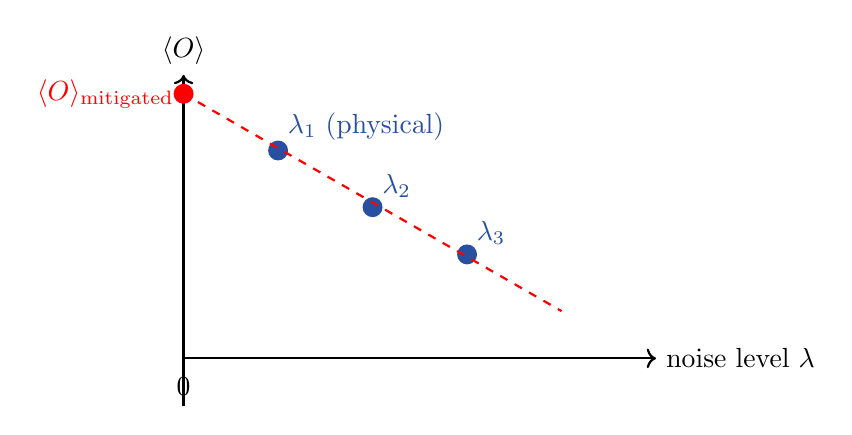
\begin{tikzpicture}[scale=1.2]
    \draw[->, thick] (0,0) -- (5,0) node[right] {noise level $\lambda$};
    \draw[->, thick] (0,-0.5) -- (0,3) node[above] {$\langle O \rangle$};

    % data points
    \fill[circuitblue] (1,2.2) circle (3pt) node[above right] {$\lambda_1$ (physical)};
    \fill[circuitblue] (2,1.6) circle (3pt) node[above right] {$\lambda_2$};
    \fill[circuitblue] (3,1.1) circle (3pt) node[above right] {$\lambda_3$};

    % extrapolation line
    \draw[dashed, red, thick] (0,2.8) -- (4,0.5);
    \fill[red] (0,2.8) circle (3pt) node[left] {$\langle O \rangle_{\text{mitigated}}$};

    % zero noise label
    \node[below] at (0,-0.1) {$0$};
\end{tikzpicture}
\end{center}

\subsection{Noise Amplification Methods}

\textbf{method 1: pulse stretching.} physically stretch the gate pulses by a factor $c > 1$. this increases the time the qubit is exposed to decoherence, effectively scaling the noise by $c$.

\textbf{method 2: unitary folding.} replace each gate $G$ with $G \cdot G^\dagger \cdot G$ (which is mathematically identical to $G$ but takes 3x the circuit depth). more generally, fold $n$ times: $G(G^\dagger G)^n$. the noise level scales roughly as $(2n+1) \times$ the original noise.

\begin{center}
\begin{quantikz}
\lstick{original:} & \gate{G} & \qw \\
\lstick{1-fold:} & \gate{G} & \gate{G^\dagger} & \gate{G} & \qw \\
\lstick{2-fold:} & \gate{G} & \gate{G^\dagger} & \gate{G} & \gate{G^\dagger} & \gate{G} & \qw
\end{quantikz}
\end{center}

\subsection{Extrapolation Methods}

\begin{definition}
given noisy expectation values at noise levels $\lambda_1, \lambda_2, \ldots, \lambda_k$, extrapolate to $\lambda = 0$:

\textbf{linear extrapolation} (Richardson, 2 noise levels):
\[
\langle O \rangle_{\text{mitigated}} = \frac{c \langle O \rangle_{\lambda_1} - \langle O \rangle_{c\lambda_1}}{c - 1}
\]

\textbf{polynomial extrapolation} ($k$ noise levels): fit a degree-$(k-1)$ polynomial through the $k$ data points and evaluate at $\lambda = 0$.

\textbf{exponential extrapolation}: fit $\langle O \rangle(\lambda) = a e^{-b\lambda} + c$ and evaluate at $\lambda = 0$. often more physically motivated for depolarizing noise.
\end{definition}

\begin{example}
linear extrapolation with noise amplification factor $c = 3$:

suppose $\langle O \rangle_{\lambda} = 0.6$ (physical noise) and $\langle O \rangle_{3\lambda} = 0.2$ (3x noise).

\[
\langle O \rangle_{\text{mitigated}} = \frac{3 \times 0.6 - 0.2}{3 - 1} = \frac{1.8 - 0.2}{2} = 0.8
\]

if the true noiseless value is $0.85$, weve gone from an error of $0.25$ to an error of $0.05$.
\end{example}

\begin{keypoint}
ZNE tradeoffs:
\begin{itemize}
    \item \textbf{pros}: simple to implement, no knowledge of the noise model needed, works with any circuit
    \item \textbf{cons}: increases variance (need more shots), assumes noise scales predictably, extrapolation can be inaccurate for complex noise models
    \item \textbf{shot overhead}: roughly $O(c^2)$ more shots needed to maintain the same statistical precision at noise level $c\lambda$
\end{itemize}
\end{keypoint}

%% ========================================================
\section{Probabilistic Error Cancellation (PEC)}
%% ========================================================

\subsection{The Idea}

PEC is more principled than ZNE but requires knowledge of the noise model. the idea:

\begin{enumerate}
    \item characterize the noise channel $\mathcal{E}$ for each gate (via tomography)
    \item express the ideal gate as a linear combination of noisy implementable operations:
    \[
    \mathcal{U}_{\text{ideal}} = \sum_i \eta_i \mathcal{O}_i
    \]
    where $\mathcal{O}_i$ r operations u can actually run on hardware and $\eta_i$ r real coefficients (can be negative)
    \item sample from this decomposition probabilistically and correct using importance sampling
\end{enumerate}

\begin{definition}
the \textbf{quasi-probability decomposition} of the ideal channel $\mathcal{U}$ given noisy channel $\mathcal{E}$:
\[
\mathcal{U} = \sum_i \eta_i \mathcal{B}_i
\]
where $\mathcal{B}_i$ r ``basis operations'' (noisy gates followed by additional pauli gates). the coefficients $\eta_i$ can be negative (hence ``quasi-probability'').
\end{definition}

\begin{keypoint}
PEC properties:
\begin{itemize}
    \item \textbf{unbiased}: gives the exact noiseless answer in expectation (no extrapolation assumptions)
    \item \textbf{cost}: the sampling overhead is $\gamma^2$ where $\gamma = \sum_i |\eta_i|$ is the 1-norm of the quasi-probability distribution. $\gamma$ grows exponentially with circuit depth for general noise.
    \item \textbf{requirement}: need a good characterization of the noise model for each gate
\end{itemize}
for a circuit with $d$ noisy gates, each with per-gate overhead $\gamma_i$: total overhead $= \prod_i \gamma_i^2$. if $\gamma_i \approx 1 + \epsilon$, total overhead $\approx e^{2d\epsilon}$. exponential in circuit depth.
\end{keypoint}

\subsection{PEC in Practice}

\begin{example}
suppose the ideal gate is $R_z(\theta)$ but the actual implementation has a small depolarizing error:
\[
\mathcal{E}(\rho) = (1-p)R_z(\theta)\rho R_z(\theta)^\dagger + \frac{p}{3}(X R_z(\theta)\rho R_z(\theta)^\dagger X + Y \ldots + Z \ldots)
\]

the quasi-probability decomposition is:
\[
\mathcal{U}_{\text{ideal}} = \frac{1}{1-p}\mathcal{E} - \frac{p}{3(1-p)}(\mathcal{E} \circ \mathcal{X} + \mathcal{E} \circ \mathcal{Y} + \mathcal{E} \circ \mathcal{Z})
\]

where $\mathcal{X}(\rho) = X\rho X$, etc. the 1-norm overhead: $\gamma = \frac{1+p}{1-p} \approx 1 + 2p$ for small $p$.
\end{example}

%% ========================================================
\section{Measurement Error Mitigation}
%% ========================================================

\subsection{The Calibration Matrix Approach}

measurement errors r often the easiest to characterize and mitigate. the idea:

\begin{enumerate}
    \item prepare each computational basis state $\ket{x}$ (e.g., $\ket{00}, \ket{01}, \ket{10}, \ket{11}$)
    \item measure many times to build a \textbf{calibration matrix} $A$ where $A_{ij} = P(\text{measure } i \,|\, \text{prepared } j)$
    \item given noisy measurement results $\vec{p}_{\text{noisy}}$, recover the ideal results: $\vec{p}_{\text{ideal}} = A^{-1}\vec{p}_{\text{noisy}}$
\end{enumerate}

\begin{definition}
the \textbf{calibration matrix} for $n$ qubits is a $2^n \times 2^n$ matrix:
\[
A_{ij} = P(\text{measure outcome } i \,|\, \text{state is } j)
\]
each column sums to 1 (its a stochastic matrix). for perfect measurements, $A = I$.
\end{definition}

\begin{example}
for 2 qubits, prepare and measure each of $\ket{00}, \ket{01}, \ket{10}, \ket{11}$:
\[
A = \begin{pmatrix} 0.95 & 0.02 & 0.03 & 0.01 \\ 0.03 & 0.93 & 0.01 & 0.04 \\ 0.01 & 0.03 & 0.94 & 0.02 \\ 0.01 & 0.02 & 0.02 & 0.93 \end{pmatrix}
\]

if noisy measurement gives $\vec{p}_{\text{noisy}} = (0.45, 0.05, 0.05, 0.45)$:
\[
\vec{p}_{\text{ideal}} \approx A^{-1}\vec{p}_{\text{noisy}} \approx (0.47, 0.03, 0.03, 0.47)
\]
\end{example}

\begin{keypoint}
practical issues with measurement mitigation:
\begin{itemize}
    \item the calibration matrix is $2^n \times 2^n$ --- exponential in the number of qubits. for $n > 10$, u cant even store it
    \item \textbf{solution}: assume measurement errors r independent (or correlated only between neighbors). then the calibration matrix is a tensor product of small matrices: $A = A_1 \otimes A_2 \otimes \cdots$
    \item $A^{-1}$ can produce negative probabilities --- need constrained optimization (least squares with non-negativity constraints)
    \item calibration drifts over time --- need to recalibrate regularly
\end{itemize}
\end{keypoint}

\subsection{Tensored Mitigation}

for $n$ qubits with independent measurement errors, each qubit $i$ has a $2 \times 2$ calibration matrix:
\[
A_i = \begin{pmatrix} 1 - p_{0|1}^{(i)} & p_{0|1}^{(i)} \\ p_{1|0}^{(i)} & 1 - p_{1|0}^{(i)} \end{pmatrix}
\]

the full calibration matrix is $A = A_1 \otimes A_2 \otimes \cdots \otimes A_n$ and its inverse is $A^{-1} = A_1^{-1} \otimes \cdots \otimes A_n^{-1}$. this only requires $2n$ calibration circuits instead of $2^n$.

%% ========================================================
\section{Dynamical Decoupling}
%% ========================================================

\subsection{The Idea}

\begin{definition}
\textbf{dynamical decoupling} (DD) is a technique to suppress decoherence during idle periods by applying fast pulses that ``average out'' the environment's effect.
\end{definition}

when a qubit is idle (waiting for other operations), it decoheres. DD fights this by inserting sequences of pulses that refocus the qubit's evolution.

\subsection{Echo Sequences}

the simplest DD sequence is the \textbf{spin echo} (Hahn echo):

\begin{center}
\begin{quantikz}
\lstick{$\ket{\psi}$} & \qw & \gate{\text{wait } \tau/2} & \gate{X} & \gate{\text{wait } \tau/2} & \qw
\end{quantikz}
\end{center}

\begin{intuition}
heres how it works. during the first wait period, the qubit picks up a random phase $\phi$ from environmental noise: $\ket{\psi} \to e^{i\phi Z}\ket{\psi}$. the $X$ pulse flips the qubit, effectively negating the phase. during the second wait period, the qubit picks up approximately the same phase $\phi$ again (assuming the noise is slow compared to $\tau$). but now it adds to $-\phi$, canceling out:

$e^{i\phi Z} \cdot X \cdot e^{i\phi Z}\ket{\psi} \approx X\ket{\psi}$ (undone by a final $X$ or tracked in software).

the net effect: low-frequency noise is canceled.
\end{intuition}

\subsection{Advanced DD Sequences}

more sophisticated sequences suppress higher-order noise:

\textbf{CPMG} (Carr-Purcell-Meiboom-Gill): $\tau - X - 2\tau - X - 2\tau - X - \cdots - X - \tau$

\textbf{XY4}: alternates X and Y pulses: $X - Y - X - Y$. suppresses noise in all directions.

\textbf{Uhrig DD (UDD)}: optimally placed pulses (not equally spaced) for specific noise spectra.

\begin{keypoint}
DD on real hardware:
\begin{itemize}
    \item IBM Quantum automatically applies DD during idle periods in circuits
    \item typical improvement: 2x--5x reduction in decoherence during idle times
    \item limitations: pulses themselves r imperfect and add small errors; doesnt help during active gates
    \item cost: zero qubit overhead, minimal circuit depth overhead (just extra single-qubit gates)
\end{itemize}
\end{keypoint}

%% ========================================================
\section{Randomized Compiling}
%% ========================================================

\subsection{The Problem with Coherent Errors}

coherent errors (systematic over/under-rotation of gates) r particularly nasty bcs they accumulate \textbf{quadratically} with circuit depth:
\[
\text{coherent error after } d \text{ gates} \sim (d\epsilon)^2
\]

compared to incoherent (random) errors which accumulate \textbf{linearly}: $\sim d\epsilon$.

\begin{definition}
\textbf{randomized compiling} (RC) converts coherent errors into incoherent errors by randomly ``twirling'' each gate. the idea: insert random pauli gates before and after each gate, choosing the paulis so that the ideal circuit is unchanged but the coherent errors r randomized.
\end{definition}

\subsection{How It Works}

for each gate $G$ in the circuit:
\begin{enumerate}
    \item randomly choose pauli gates $P_{\text{before}}$ and compute $P_{\text{after}} = G \cdot P_{\text{before}} \cdot G^\dagger$ (so that the ideal circuit is $P_{\text{after}} \cdot G \cdot P_{\text{before}} = G$)
    \item absorb $P_{\text{before}}$ into the preceding gate and $P_{\text{after}}$ into the following gate
    \item run many randomized versions and average the results
\end{enumerate}

\begin{center}
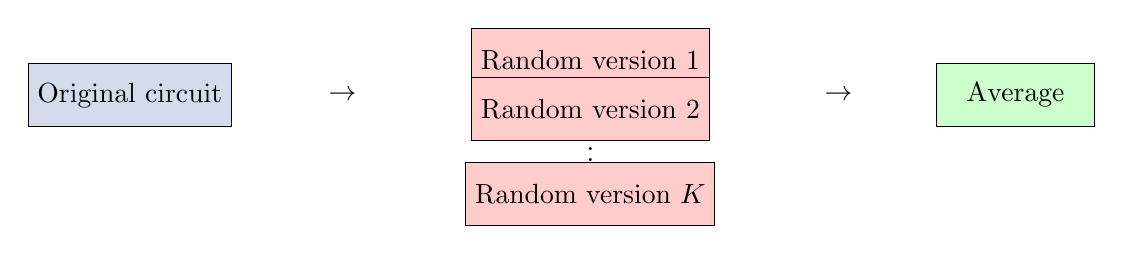
\begin{tikzpicture}[scale=0.9]
    \node[draw, fill=circuitblue!20, minimum width=2cm, minimum height=0.8cm] at (0,0) {Original circuit};
    \node at (3,0) {$\to$};
    \node[draw, fill=red!20, minimum width=2.5cm, minimum height=0.8cm] at (6.5,0.5) {Random version 1};
    \node[draw, fill=red!20, minimum width=2.5cm, minimum height=0.8cm] at (6.5,-0.2) {Random version 2};
    \node at (6.5,-0.8) {$\vdots$};
    \node[draw, fill=red!20, minimum width=2.5cm, minimum height=0.8cm] at (6.5,-1.4) {Random version $K$};
    \node at (10,0) {$\to$};
    \node[draw, fill=green!20, minimum width=2cm, minimum height=0.8cm] at (12.5,0) {Average};
\end{tikzpicture}
\end{center}

\begin{keypoint}
randomized compiling benefits:
\begin{itemize}
    \item converts coherent errors (quadratic accumulation) to incoherent errors (linear accumulation)
    \item the effective noise channel becomes a pauli channel (much easier to analyze and mitigate with ZNE or PEC)
    \item minimal overhead: just extra single-qubit paulis (fast, high-fidelity gates)
    \item often combined with ZNE or PEC for maximum benefit
\end{itemize}
\end{keypoint}

%% ========================================================
\section{Practical Implications for QML}
%% ========================================================

\subsection{Circuit Depth Limits}

\begin{keypoint}
noise fundamentally limits wt QML can do on NISQ hardware:
\begin{enumerate}
    \item \textbf{circuit depth}: with 2-qubit gate fidelity $\sim 99\%$, useful circuit depth is $\sim 50$--$100$ gates. this limits the expressibility of quantum models.
    \item \textbf{number of qubits}: more qubits $=$ more noise sources $=$ faster decoherence. current useful range: $\sim 10$--$50$ qubits.
    \item \textbf{number of shots}: error mitigation techniques (especially PEC) require exponentially more shots as circuit depth increases. this limits practical circuit depth even further.
    \item \textbf{parameter optimization}: noisy gradients make training harder. noise-induced barren plateaus can make the loss landscape flat.
\end{enumerate}
\end{keypoint}

\subsection{Noise-Aware QML Design}

\begin{keypoint}
strategies for building QML models that work on noisy hardware:
\begin{itemize}
    \item use \textbf{hardware-efficient ansatze} --- circuits that match the native gate set and connectivity of the hardware
    \item keep circuits \textbf{shallow} --- fewer gates means less noise
    \item use \textbf{local cost functions} --- they r less affected by noise than global cost functions (Cerezo et al. 2021)
    \item apply \textbf{measurement error mitigation} --- its cheap and always helps
    \item use \textbf{ZNE} for expectation value estimation in variational circuits
    \item consider \textbf{error-robust ansatze} --- circuit designs that r naturally less sensitive to certain error types
    \item \textbf{noise-aware training}: include noise models in the classical simulation during hyperparameter tuning
\end{itemize}
\end{keypoint}

\subsection{The Sampling Overhead Problem}

\begin{intuition}
heres the fundamental tension in NISQ QML:

\textbf{expressibility} needs deep circuits $\to$ more noise $\to$ need more error mitigation $\to$ need exponentially more measurement shots $\to$ kills any quantum advantage.

\textbf{noise robustness} needs shallow circuits $\to$ limited expressibility $\to$ might not be more powerful than classical models.

this is the NISQ dilemma. finding the sweet spot --- circuits deep enough to be useful but shallow enough to be mitigatable --- is the central challenge of practical QML.
\end{intuition}

%% ========================================================
\section{Comparing Error Mitigation Techniques}
%% ========================================================

\begin{center}
\begin{tabular}{l|c|c|c|c}
technique & bias & overhead & noise model & complexity \\
\hline
ZNE & biased & moderate & not needed & easy \\
PEC & unbiased & exponential & required & moderate \\
meas. mitigation & unbiased & linear & partial & easy \\
dynamical decoupling & N/A & minimal & not needed & easy \\
randomized compiling & biased & moderate & not needed & moderate
\end{tabular}
\end{center}

\begin{keypoint}
in practice, the best approach combines multiple techniques:
\begin{enumerate}
    \item \textbf{randomized compiling}: tailors coherent errors into incoherent ones (apply always)
    \item \textbf{dynamical decoupling}: during idle times (apply always, near-free)
    \item \textbf{measurement error mitigation}: on the readout (apply always, cheap)
    \item \textbf{ZNE or PEC}: on the expectation values (apply when u can afford the shot overhead)
\end{enumerate}
this layered approach gives the best results on current hardware.
\end{keypoint}

%% ========================================================
\section{Noise Characterization Techniques}
%% ========================================================

before u can mitigate noise, u need to know wt the noise is. here r the main characterization techniques:

\subsection{Quantum State Tomography (QST)}

\begin{definition}
\textbf{QST} fully reconstructs the density matrix of an $n$-qubit state by measuring in multiple bases. for $n$ qubits, u need at least $3^n$ measurement settings (all combinations of X, Y, Z measurements on each qubit) and $4^n - 1$ parameters to estimate.
\end{definition}

QST is exponentially expensive --- only practical for $\lesssim 10$ qubits. but its the gold standard for verifying small quantum states.

\subsection{Quantum Process Tomography (QPT)}

\begin{definition}
\textbf{QPT} fully characterizes a quantum channel by preparing a complete set of input states, sending them through the channel, and doing QST on each output. for $n$ qubits: prepare $4^n$ input states, do QST on each $\to$ $O(16^n)$ total experiments.
\end{definition}

even more expensive than QST. only practical for 1--2 qubit gates.

\subsection{Randomized Benchmarking (RB)}

\begin{definition}
\textbf{randomized benchmarking} estimates the average gate fidelity without full process tomography:
\begin{enumerate}
    \item apply a random sequence of $m$ clifford gates
    \item apply the inverse of the entire sequence
    \item measure the probability of returning to the initial state
    \item repeat for various sequence lengths $m$
    \item fit the decay: $F(m) = A \cdot p^m + B$
    \item the average error per gate: $r = (1-p)(1 - 1/2^n)$
\end{enumerate}
\end{definition}

\begin{intuition}
RB is efficient bcs it only estimates a single number (average fidelity) rather than the full process matrix. the random clifford twirling converts any noise into depolarizing noise, and the depolarizing parameter decays exponentially with sequence length. the decay rate tells u the average error per gate.

RB is wt hardware vendors use to report gate fidelities. when IBM says their CNOT fidelity is 99.5\%, thats from RB.
\end{intuition}

%% ========================================================
\section{Advanced Topic: Twirling}
%% ========================================================

\begin{definition}
\textbf{twirling} is a technique that simplifies a noise channel by averaging over a group of unitaries:
\[
\mathcal{E}_{\text{twirled}}(\rho) = \frac{1}{|G|}\sum_{g \in G} g^\dagger \mathcal{E}(g \rho g^\dagger) g
\]

\textbf{pauli twirling}: average over the pauli group. converts any noise channel into a pauli channel (only diagonal elements survive in the pauli transfer matrix).

\textbf{clifford twirling}: average over the clifford group. converts any noise channel into a depolarizing channel.
\end{definition}

\begin{intuition}
twirling is the theoretical foundation behind both randomized benchmarking and randomized compiling. by averaging over random unitaries, u ``symmetrize'' the noise into a simpler form. pauli twirling gives u a pauli channel (easy to work with). clifford twirling gives u depolarizing noise (the simplest possible noise model).

this is deeply connected to representation theory --- the twirled channel lives in the commutant of the twirling group, and for the pauli/clifford groups, this commutant has a simple structure.
\end{intuition}

%% ========================================================
\section{Summary}
%% ========================================================

\begin{keypoint}
key takeaways from both noise lectures:
\begin{enumerate}
    \item QEC is the ultimate solution but requires $\sim 1000$x qubit overhead. not practical yet.
    \item for NISQ: use error mitigation techniques (ZNE, PEC, measurement mitigation, DD, RC)
    \item ZNE: amplify noise, extrapolate to zero. simple but biased.
    \item PEC: unbiased but exponential sampling overhead. needs noise characterization.
    \item measurement mitigation: calibration matrix approach. cheap and effective.
    \item dynamical decoupling: free lunch for idle qubits. always use it.
    \item randomized compiling: converts coherent errors to incoherent. always helps.
    \item the NISQ dilemma: need deep circuits for expressibility, but noise kills deep circuits. finding the sweet spot is the central challenge.
    \item for QML specifically: noise limits circuit depth, adds training difficulty, and can create noise-induced barren plateaus. noise-aware design is essential.
\end{enumerate}
\end{keypoint}

with the noise story complete, were ready to move on to the ML side of things. next: classical machine learning foundations.

\end{document}
